\section{Method: \boldmath \ourmethod}
\label{sec:method}

% Section~\ref{sec:diagnosis} shows that stale rollouts remain useful under relaxed clipping, but
% high-staleness optimization becomes unstable when negative-advantage trajectories
% cross an off-support boundary. With this observation

Section~\ref{sec:diagnosis} shows that high-staleness rollouts can retain useful
learning signal once their localized instability is controlled. This staleness
tolerance allows us to safely pursue high-staleness training, where a large
static rollout dataset supports many optimizer updates. As a result, we can
reduce frequent rollout refreshes and translate algorithmic tolerance into
system efficiency.

\paragraph{\boldmath \ourmethod{}.} We propose a staged training framework that separates rollout generation and
policy optimization into large-$\mu$ phases. Instead of tightly interleaving
generation and optimization as in standard GRPO, \ourmethod{} generates
rollouts in bulk and then performs many policy updates on the resulting static
dataset. Each stage consists of two phases:

\begin{figure*}[!h]
\vspace{-1.2em}
    \centering
    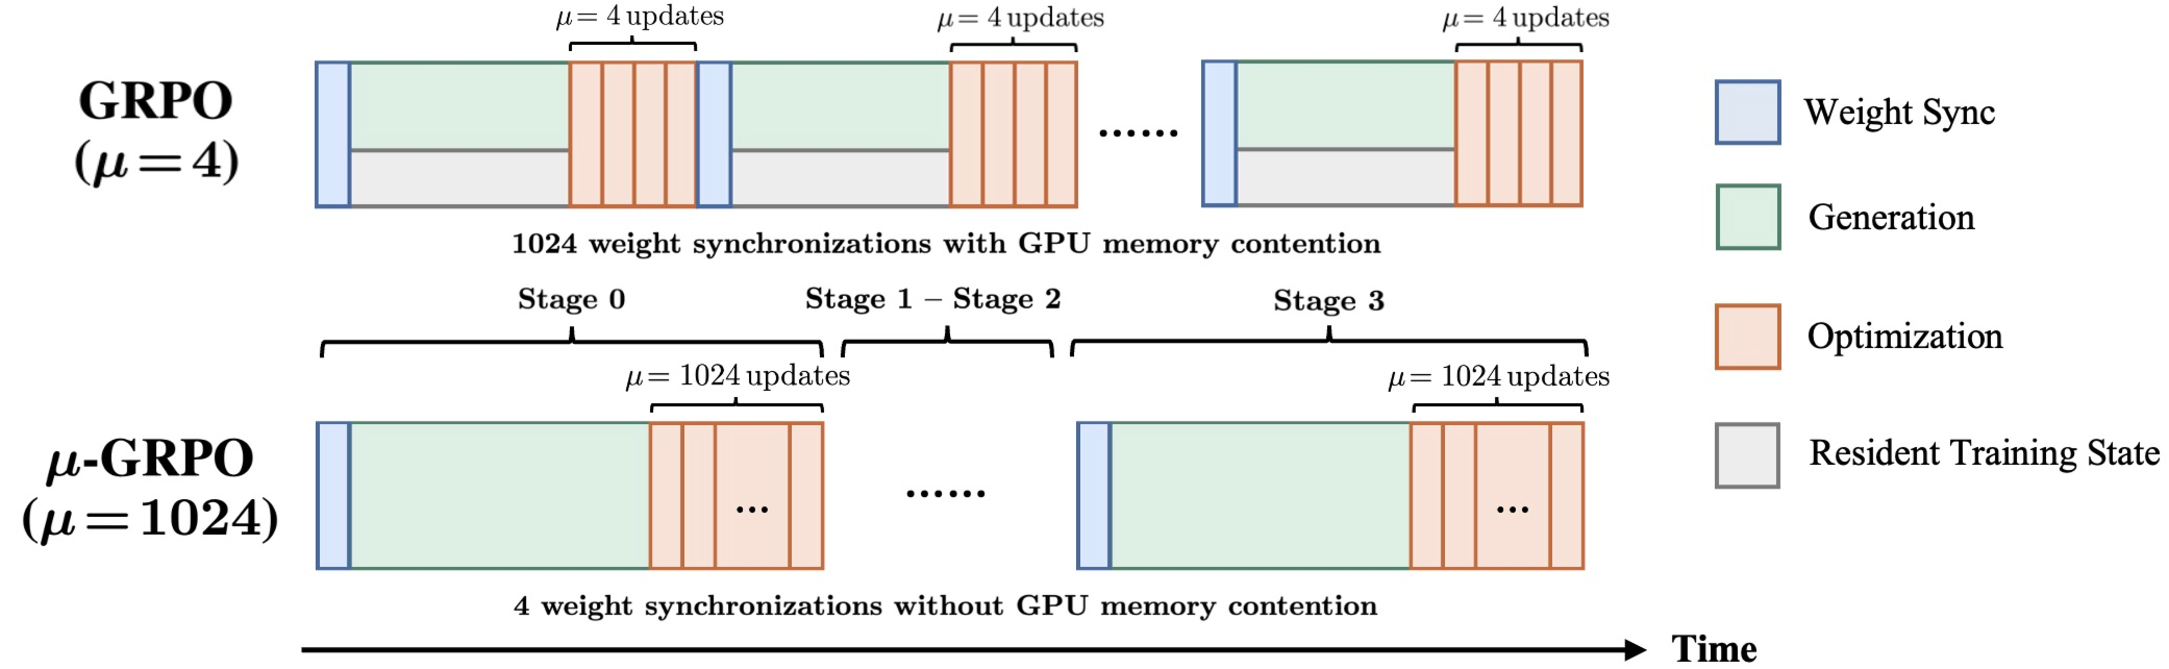
\includegraphics[width=0.95\textwidth]{figures/framework.pdf}
    \caption{
\textbf{System-level execution of standard GRPO and \boldmath\ourmethod.}
Over 4096 model updates, standard GRPO with $\mu\!=\!4$ requires 1024 rollout
refreshes and weight synchronizations, while \ourmethod{} with $\mu\!=\!1024$
requires only four. Large-stage rollout generation reduces synchronization
overhead and avoids GPU memory contention during generation.
    }
    \label{fig:framework}
\vspace{-1.5em}
\end{figure*} 
\paragraph{Phase 1: High-Throughput Rollout Generation.}
\label{paragraph:phase1}
At the beginning of each stage $k$, we freeze the current policy as the rollout
policy $\beta_k$ and use it only for rollout generation. Specifically, for the
first stage, we initialize the rollout policy from the base model,
$\beta_0 \leftarrow \pi_{\text{base}}$; for later stages, $\beta_k$ is obtained
by freezing the policy after the optimization phase of stage $k-1$. 
Given the stage prompt set $\mathcal{X}_k=\{x_i\}_{i=1}^{B_{\mathrm{train}}}$,
the rollout policy $\beta_k$ samples a response group
$\mathcal Y_i=\{y_{i,g}\}_{g=1}^G$ for each prompt $x_i$.
For each generated response $y=(a_1,\ldots,a_T)$ to prompt $x$, we compute its
group-normalized advantage $A$ as in Eq.~\ref{eq:grpo-adv} and store tokenwise
behavior log-probabilities $b_{1:T}$ with
$b_t=\log\beta_k(a_t\mid x,a_{<t})$.
The resulting static rollout dataset is
\[
\mathcal D_k=\{(x_i, y, A, b_{1:T}) : x_i\in\mathcal X_k,\; y\in\mathcal Y_i\}.
\]
The frozen rollout engine emits behavior log-probabilities during decoding, avoiding an additional behavior-policy forward pass. Once rollout generation is complete, the rollout engine can be
released from memory, and $\mathcal D_k$ is passed to the optimization phase.


\paragraph{Phase 2: Policy Optimization with Large \boldmath $\mu$.}
\label{paragraph:phase2}

The policy is then optimized on the static rollout dataset $\mathcal D_k$ for $\mu=B_{\mathrm{train}}/B_{\mathrm{mini}}$ updates before the next rollout
stage. By making $B_{\mathrm{train}}$ large, \ourmethod{} operates with
$\mu$ on the order of thousands, reusing the same behavior policy over many updates. During optimization, $\beta_k$ is fixed and its behavior log-probabilities are already stored, so the rollout engine need not remain resident. For a token $a_t$ in response $y$ to prompt $x$, with stored behavior log-probability $b_t$, we compute the importance ratio as
\[
    \rho_t(\theta)
    =
    \exp\left(
        \log \pi_\theta(a_t\mid x,a_{<t}) - b_t
    \right).
\]
Motivated by the analysis in \cref{sec:diagnosis}, \ourmethod{} applies
\textit{negative-advantage veto} before the GRPO update. For each negative-advantage
response $y$, the veto rule checks whether any token satisfies
$\rho_t(\theta)<\tau_c$. We consider three veto scopes that contain the diagnosed non-trigger suffix
$\mathcal H_\kappa$: $\mathcal H_\kappa$, $\mathcal S_\kappa$, and
$\mathcal S_{\mathrm{seq}}$. We use $\mathcal S_{\mathrm{seq}}$ by default for simplicity and robustness, and ablate the scope choice in Appendix~\ref{app:nav_scope_ablation}. Under this default, once a trigger is detected, the entire response is masked. Thus, in the objective below, $m_{t}(\theta)$ is zero
for all tokens in a triggered negative-advantage response and equals one otherwise.
The mask is recomputed at each update and is not differentiated through. 

With this mask, we optimize a relaxed clipped GRPO objective with clipping range $[0,5]$:
% \[
% \begin{aligned}
%     J_{\mu\text{-GRPO}}(\theta)
%     =
%     \mathbb{E}_{\mathcal{B}\sim\mathcal{D}_k}
%     \Bigg[
%     \frac{1}{|\mathcal{B}|}
%     \sum_{(i,g)\in \mathcal{B}}
%     \frac{1}{T_{i,g}}
%     \sum_{t=1}^{T_{i,g}}
%     m_{i,g,t}(\theta)
%     \min\Big(
%         \rho_{i,g,t}(\theta) A_{i,g},
%         \operatorname{clip}(\rho_{i,g,t}(\theta),0,5) A_{i,g}
%     \Big)
%     \Bigg].
% \end{aligned}
% \]   
\[
J_{\mu\text{-GRPO}}(\theta)
=
\mathbb{E}_{\mathcal B\sim\mathcal D_k}
\left[
\frac{1}{|\mathcal B|}
\sum_{(x,y,A,b_{1:T})\in\mathcal B}
\frac{1}{T}
\sum_{t=1}^{T}
m_t(\theta)
\min\left(
\rho_t(\theta)A,
\operatorname{clip}(\rho_t(\theta),0,5)A
\right)
\right].
\]


% The implemented loss is $-J_{\mu\text{-GRPO}}(\theta)$. 

\paragraph{Multi-Stage \boldmath $\mu$-GRPO.}
\label{sec:multistage}
\setlength{\columnsep}{10pt}
\begin{wrapfigure}{r}{0.45\linewidth}
\vspace{-1.35em}
\centering
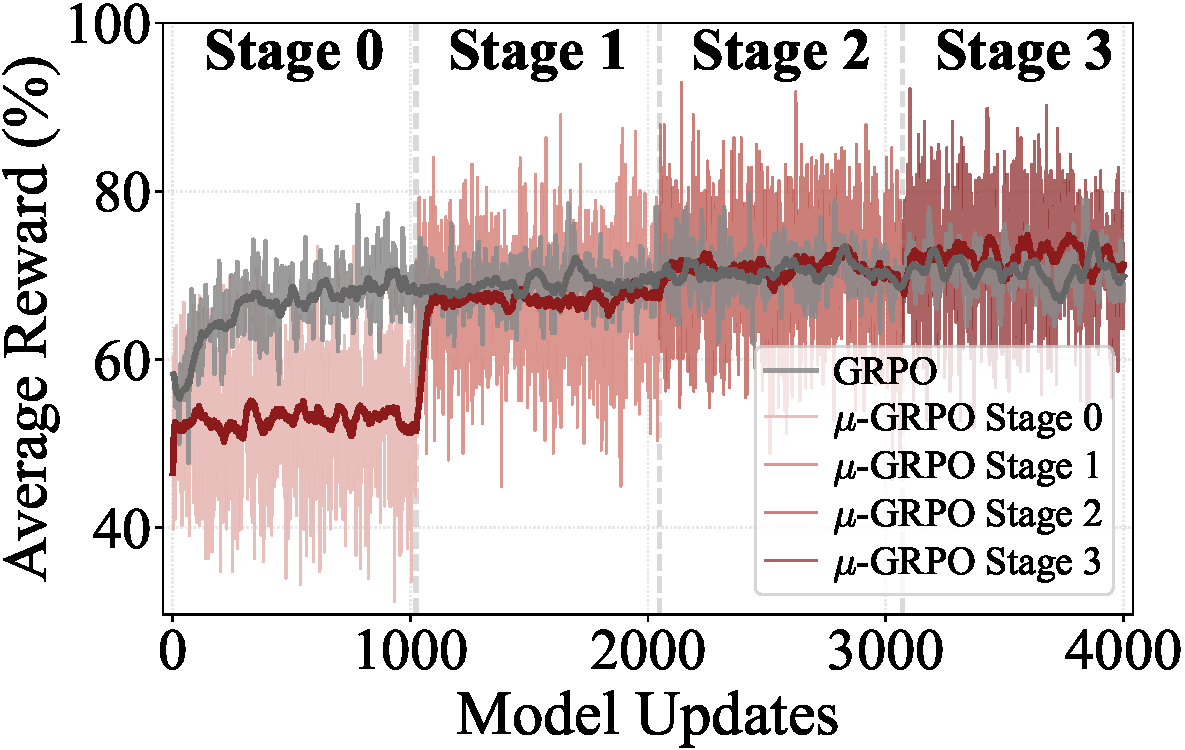
\includegraphics[width=\linewidth]{figures/reward.pdf}
\vspace{-1.6em}
\caption{
\textbf{Training-set reward dynamics} on DeepSeek-7B. Bold lines are smoothed. 
% \ourmethod{} maintains stable reward improvement across stages
% despite larger variance from high rollout staleness.
}
\label{fig:reward}
\vspace{-12pt}
\end{wrapfigure}

Both standard GRPO and $\mu$-GRPO can be viewed as repeated
generation--optimization cycles, as illustrated in \cref{fig:framework}. The key difference is the scale of each cycle:
standard GRPO refreshes the behavior policy after small rollout batches, keeping
$\mu$ low, whereas $\mu$-GRPO generates a large static rollout dataset and
performs many updates before the next rollout stage. The two-phase procedure above
defines one such large-$\mu$ stage. After stage $k$ consumes $\mathcal{D}_k$, the
updated policy is frozen as the rollout policy for stage $k+1$, and a fresh
dataset $\mathcal{D}_{k+1}$ is generated.
This design separates two timescales: within each stage, the rollout policy stays fixed for many updates to amortize generation; across stages, it is refreshed
only a few times to improve rollout quality. As shown in
\cref{fig:reward,fig:teaser}, this sparse refresh schedule improves training-set
reward across stages and translates the large-$\mu$ efficiency gain into stable
evaluation performance.

\paragraph{System-Level Efficiency.}
\label{sec:method_efficiency}
Figure~\ref{fig:framework} compares the execution schedules of standard GRPO and \ourmethod{} over 4096 model updates. Standard GRPO with $\mu=4$ requires 1024 rollout refreshes and weight synchronizations between a high-throughput
inference engine, such as vLLM~\citep{kwon2023efficientmemorymanagementlarge} or
SGLang~\citep{zheng2024sglangefficientexecutionstructured}, and a sharded
training engine, such as
FSDP~\citep{zhao2023pytorchfsdpexperiencesscaling} or
Megatron-LM~\citep{DBLP:journals/corr/abs-1909-08053}. Each refresh can incur sharded-parameter materialization, transfer to the rollout engine, and inference-layout conversion. Frequent alternation also creates GPU memory contention: to switch quickly between generation and optimization, systems often keep model parameters and optimizer states resident during rollout. This reduces memory available for high-throughput inference.


\ourmethod{} reduces both costs by operating at large rollout staleness
($\mu\!=\!1024$):
Over 4096 model updates, it performs only four rollout stages and
weight synchronizations. Within each stage, rollout generation is executed as a
standalone phase: the frozen rollout policy generates a large static dataset,
after which the rollout engine can be released and the trainer consumes the data
using stored behavior log-probability anchors. With only a
few generation--optimization switches, training state need not remain co-resident
during rollout, leaving more device memory for larger rollout batches and higher decoding parallelism. Large-$\mu$
training therefore turns GRPO's staleness tolerance into lower synchronization
overhead, lower memory contention, and higher rollout throughput.
